\documentclass{article}

\usepackage{amsmath}
\usepackage{amssymb}
\usepackage{mathrsfs}
\usepackage{amsthm}
\usepackage{textcomp}
\usepackage{xcolor}
\usepackage{graphicx}
\usepackage{enumerate}
\usepackage{mathtools}
\usepackage{hyperref}
\usepackage[title]{appendix}
\usepackage{subfigure}
\usepackage{bm}
\usepackage[top=2cm, bottom=2cm, left=2cm, right=3cm]{geometry} % pr modifier les dimensions des marges etc.
\usepackage{dsfont}
\usepackage{caption}
\usepackage{todonotes}
\usepackage{framed}
\usepackage{wrapfig}
\usepackage{tikz,pgfplots}
 \pgfplotsset{compat=1.9}

\newtheorem{thm}{Theorem}
\newtheorem{prop}[thm]{Proposition}
\newtheorem{cor}[thm]{Corollary}
\newtheorem{conj}[thm]{Conjecture}
\newtheorem{defi}[thm]{Definition}
\newtheorem{lem}[thm]{Lemma}
\newtheorem{hypo}[thm]{Hypothesis}
\newtheorem{ass}[thm]{Assumption}

\renewcommand{\thefootnote}{\fnsymbol{footnote}}
\newcommand{\J}{{\cal J}}
\newcommand{\I}{{\cal I}}
\newcommand{\spec}{{\rm spec}}

\begin{document}

\title{Notes: melting pot about machine learning}
\author{Robin Delabays}
\date{\today}

\maketitle

\section{ML algorithms}\label{sec:ml_algo}

\subsection{Kernel methods}
See Florian's notes~\cite{Florian} and the survey~\cite{Pil14}. 

\subsection{Reservoir computing}
Good summary in~\cite{Lu17}.

\section{Observations}
Our aim is to predict the behavior of a (partially) unknown dynamical system, using algorithms of machine learning. 
We want to compare the performances of the algorithms described in Sec.~\ref{sec:ml_algo}. 
Further objective would be to evaluate how long the algorithm manage to mimic the dynamical system once it does not have real-time measurement anymore.

\subsection{LTI system}
We consider the Linear Time Invariant (LTI) system, subject to Gaussian noise, with unkown initial conditions,  
\begin{align}\label{eq:lti}
 \dot{x} &= Ax\, , & y &= Cx + \epsilon\, ,
\end{align}
where $\epsilon\sim{\cal N}(0,\sigma)$. 
If the initial conditions are $x_0$, then 
\begin{align}
 y(t) &= C\exp(At)x_0+\epsilon(t)\, .
\end{align}

We will use 
\begin{align}\label{eq:lti_params}
 A &=
 \begin{pmatrix}
  0 & 1 \\
  -0.1 & 0
 \end{pmatrix}\, ,
 & C &= 
 \begin{pmatrix}
  0 & 1
 \end{pmatrix}\, ,
 & \epsilon\sim{\cal N}(0,0.01)\, .
\end{align}

As shown by Florian, kernel methods work well for such systems, provided we know $A$ and $C$, and using pairs $\{(t_i,y(t_i)\}_{i=1,...,T}$ as training data. 
Actually, we can verify that this works quite well already for rather small $T\in\{5,...,10\}$. 

Our reservoir computer works very poorly on this specific problem (see Fig.~\ref{fig:reservoir_lti_1}), even without noise. 
The training times were taken randomly (not at fixed intervals). 
\begin{figure}
 \centering
 \includegraphics[width=.5\textwidth]{figs/reservoir_lti_1.pdf}
 \caption{Trajectory of $y$ for the LTI system Eq.~\eqref{eq:lti_params} (blue dashed line) and the reservoir computing estimation of it (orange dots). 
 Inputs are random times. 
 $N=1000$, $D=20$, $\rho=1$, $\sigma=0.01$, $\alpha=1$, $\xi=1$, $\beta=1$. }
 \label{fig:reservoir_lti_1}
\end{figure}

Our reservoir computer works much better if we gives training pairs $\{(y(t_0+k\Delta t),y(t_0+(k+\Delta k)\Delta t))\}_{k=1,...,T}$, 
i.e., system measurement with a time delay of $\Delta k\Delta t$. 
In Fig.~\ref{fig:reservoir_lti_2}, we gave the training outputs as inputs for the systems prediction, but without noise. 
When noise is added, this does not work very well anymore. 
Fig.~\ref{fig:reservoir_lti_3} gives the same estimation with noise $\epsilon\sim{\cal N}(0,0.01)$ with $\Delta k=1$. 
\begin{figure}
 \centering
 \includegraphics[width=\textwidth]{figs/reservoir_lti_2.pdf}
 \caption{Trajectory of $y$ for the LTI system Eq.~\eqref{eq:lti_params} (blue dashed line) and the reservoir computing estimation of it (orange dots). 
 Inputs are previous system's state. 
 $N=1000$, $D=20$, $\rho=1$, $\sigma=0.01$, $\alpha=1$, $\xi=1$, $\beta=1$, $\Delta k=T_{\rm simu}$. }
 \label{fig:reservoir_lti_2}
\end{figure}
\begin{figure}
 \centering
 \includegraphics[width=.5\textwidth]{figs/reservoir_lti_3.pdf}
 \caption{Same as Fig.~\ref{fig:reservoir_lti_2} with noise. 
 $N=1000$, $D=20$, $\rho=1$, $\sigma=0.01$, $\alpha=1$, $\xi=1$, $\beta=1$, $\Delta k=1$. }
 \label{fig:reservoir_lti_3}
\end{figure}

\subsection{Lorentz system}
According to~\cite{Lu17}, the Lorentz system 
\begin{align}\label{eq:lorentz}
 \dot{x} &= \sigma(y-x)\, , & \sigma &= 10\, , \\
 \dot{y} &= x(\rho-z)-y\, , & \rho &= 28\, , \\
 \dot{z} &= xy - \beta z\, , & \beta &= 8/3\, ,
\end{align}
is well predicted by reservoir computing, using the measurement of $x$ as input and the other two variables $y$ and $z$ as output. 
We verified this. 

Until now I have not been able to find a satisfying kernel to predict it using kernel methods. 
Kernels based on a basis of monomials (up to degree $4$) as well a Gaussian kernels work poorly (Fig.~\ref{fig:kernel_lorentz_1}).
\begin{figure}
 \centering
 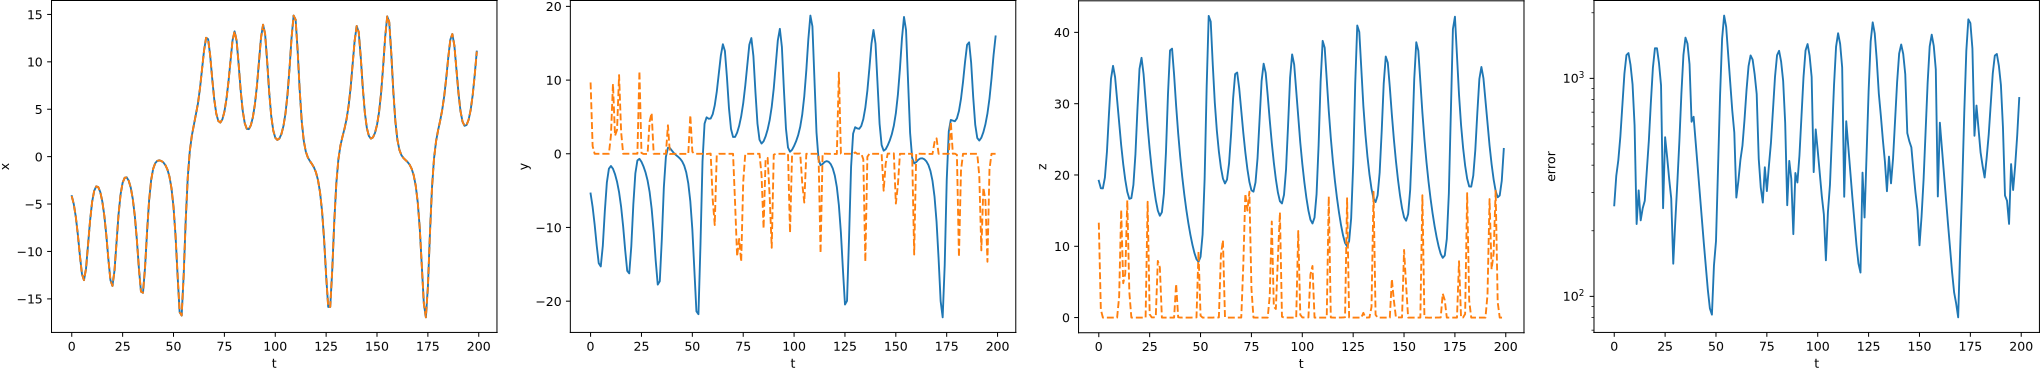
\includegraphics[width=\textwidth]{figs/kernel_lorentz_1}
 \caption{Trajectory of the Lorentz system Eq.~\eqref{eq:lorentz} (blue line) and its ``prediction'' by Gaussian kernel method (orange dashed line).
 The variable $x$ is exact because it is the input. 
 $T=5000$, $\rho=1$, $\gamma=10^{-9}$.}
 \label{fig:kernel_lorentz_1}
\end{figure}




\bibliographystyle{mystyle}
\bibliography{bibliography}

\end{document}
